\documentclass[a4paper, 12pt]{ctexart}

\usepackage{enumerate}
\usepackage{graphicx}
\usepackage{listings}
\usepackage{xcolor}
%\usepackage{fancyhdr}


% code listings
\lstdefinestyle{customc}{
	belowcaptionskip=1\baselineskip,
	breaklines=true,
	frame=L,
	xleftmargin=\parindent,
	language=C,
	showstringspaces=false,
	basicstyle=\footnotesize\ttfamily,
	keywordstyle=\bfseries\color{green!40!black},
	commentstyle=\itshape\color{purple!40!black},
	identifierstyle=\color{blue},
	stringstyle=\color{orange},
}

\lstset{basicstyle=\ttfamily\color{brown},
	showstringspaces=false,
	commentstyle=\color{red},
	keywordstyle=\color{blue}
}

%%%%%%%%%%%% author  %%%%%%%%%%%%%%%%
\author{金国栋\\
	\and
	韩涵\\
	\and
	黄文韬\\
	\and
	陈成\\
}
\title{分布与并行数据库Pard系统实验报告}
\date{\today}


%%%%%%%%%%%%%%%==============  \begin{document}  ====================%%%%%%%%%%%%%%%%%%%
\begin{document}

\maketitle%
\hspace{8em}
\begin{figure}[h]
	\centering
	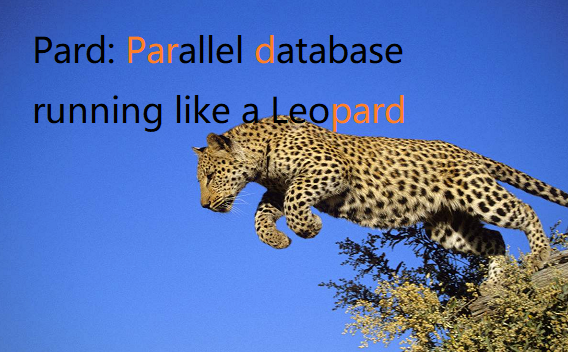
\includegraphics[width=0.7\linewidth]{figure/leopard.png}
\end{figure}

\newpage
 
\tableofcontents
 
 
\section{系统概述}
\subsection{任务描述}
本实验主要设计和实现一个面向分析的分布式数据库系统,即通过网络将多个不同的局部数据库系统连接起来,
使得用户可以通过分布式数据库管理系统达到透明性管理的目的,采用横向扩展的方式,扩展数据库系统的查询性能。

\subsection{系统需求}
\begin{enumerate}
\item 支持数据库的创建和删除。
\item 支持表的创建和删除。
\item 支持数据表的水平分片和垂直分片。
\item 支持元数据的存储和管理。
\item 支持数据从文件批量导入。
\item 支持插入记录。
\item 支持删除记录。
\item 支持SQL语句\textit{select ... from ... where ...}。
\end{enumerate}

\subsection{运行环境}
Pard系统采用Java语言开发,运行时需要Java 8以上的运行环境,目前仅支持Linux系统。
Pard采用P2P的设计思想,每个Pard Server都可以部署在集群中的任意节点上,且每个节点都可以作为主节点被客户端访问。
在我们的实验环境中,我们利用三台普通台式机搭建了一个集群,分别为pard01、pard02和pard03。
其中pard01和pard02分别部署了一个Pard Server,pard03部署了两个Pard Server。

\subsection{开发环境}
系统的开发环境主要由Git、Maven(v3.3.9+)和Java 8构成。开发的IDE包括Eclipse和Intellij IDEA。
系统利用Maven实现了代码风格的管理和代码编译、打包、自动分发的功能,方便了项目的开发过程。
\lstinline|mvn clean compile|
\lstinline[language=bash]|mvn clean package|
 
\subsection{使用说明}
Pard系统的使用说明如下:
\begin{enumerate}
\item 代码编译和打包:

切换到Pard项目的根目录,执行
\lstinline[language=bash]|mvn clean package|

\textit{pard-assembly/target}目录下的\textit{.zip}或\textit{.tar.gz}文件即为部署文件。

解压后目录结构如图\ref{release}
\begin{figure}[htbp]
	\centering
	\includegraphics[width=\linewidth]{figure/release.png}
	\caption{发布版目录结构}
	\label{fig:release}
\end{figure}

\item Pard Server的启动:
\lstinline[language=bash]|./sbin/pard-server start/run|
Pard Server的启动方式分为两种:
\begin{itemize}
	\item start: 后台启动。Pard Server进程将利用nohup后台启动。
	\item run: 前台启动。
\end{itemize}
对于后台启动的Pard Server,可以调用
\lstinline[language=bash]|./sbin/pard-server stop|
停止进程。

\item 配置文件:
\begin{itemize}
\item \textit{pard.name}: Pard Server的名称,需要保证每个Server都不相同。
\item \textit{pard.host}: Pard Server的网络IP地址。
\item \textit{pard.server.port}: Pard Server的服务端口号。客户端连接该端口。
\item \textit{pard.web.port}: Pard Server的网络端口号。
\item \textit{pard.rpc.port}: Pard Server的RPC端口。供Server之间调用。
\item \textit{pard.exchange.port}: Pard Server数据传输的端口。
\item \textit{pard.file.port}: Pard Server文件传输的端口。
\item \textit{pard.connector.host}: Pard Server连接的数据库的地址。
\item \textit{pard.connector.user}: Pard Server连接的数据库的用户名。
\item \textit{pard.connector.password}: Pard Server连接的数据库对应用户的密码。
\item \textit{pard.connector.driver}: Pard Server使用的JDBC连接的driver类。
\end{itemize}
\end{enumerate}

\subsection{项目管理}
Pard的开发利用Github进行协同,并且代码都开源在Github上。\textit{https://github.com/dbiir/pard} 
 
\section{系统架构}
Pard整体架构如图\ref{fig:archi}。用户通过命令行连接集群中的任意一个Pard Node进行交互,每个Pard Node都可以通过内置的connector连接多个SlaveDB。
通过connector的方式屏蔽底层SlaveDB的细节,这样SlaveDB可以为PostgreSQL或者MySQL等任意数据库,只需按照connector的接口开发对应的connector即可。

\begin{figure}[htbp]
	\centering
	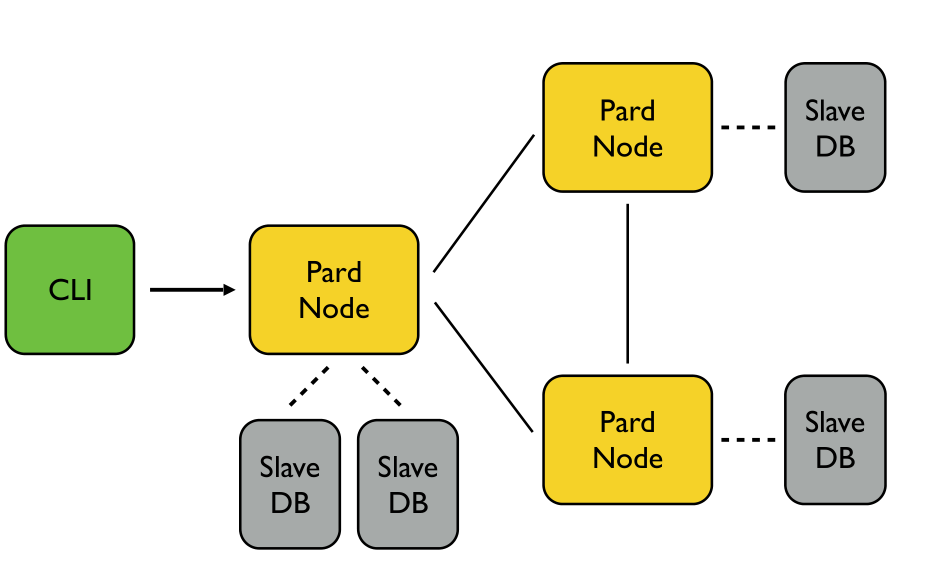
\includegraphics[width=\linewidth]{figure/architecture.png}
	\caption{Pard整体架构图}
	\label{fig:archi}
\end{figure}

Pard单个节点的架构如图\ref{fig:node1}。每个节点都有可能成为与用户直接交互的节点,应用层面诸如Client、Web UI
是用户可见的抽象层级。下面来看底层实现。Pard收到用户输入的SQL语句,转化为执行的Job,先交给SQL Parser进行SQL的语法解析,得到抽象语法树AST。
再依据查询本身特性和数据划分的特点,在SQL Optimizer模块中进行优化。然后由Job Planner制定物理的查询执行计划,并将计划交给Job scheduler,生成具体的查询执行任务,
分发给各个节点去执行,并协调任务之间执行的顺序、同步异步等。

各个节点还有存储管理模块,负责管理数据在内存中的组织形式。数据在内存中以\textit{Block}的方式组织。
节点中的通讯模块具体分两类:一类是任务的通信,使用RPC技术发送较小数据量的任务通知;
另一类是SQL执行需要的大批量数据的通信,比如节点之间的数据shuffle,我们使用Netty做大批量数据的异步传输。
元数据由各节点的Catalog模块维护,数据分布在集群中的各个节点,由分布式的KV存储系统etcd负责存储和数据的同步,etcd遵循的raft协议可以确保各个节点元数据的一致性。
节点中的Executor是本地执行器,负责执行接收到的具体的查询任务,并调用Connetor与本地连接的数据库进行交互。
NodeKeeper模块负责集群中节点状态的维护,每个Pard Server启动的时候都需要向NodeKeeper注册,并在进程结束的时候通知NodeKeeper。

\begin{figure}[htbp]
	\centering
	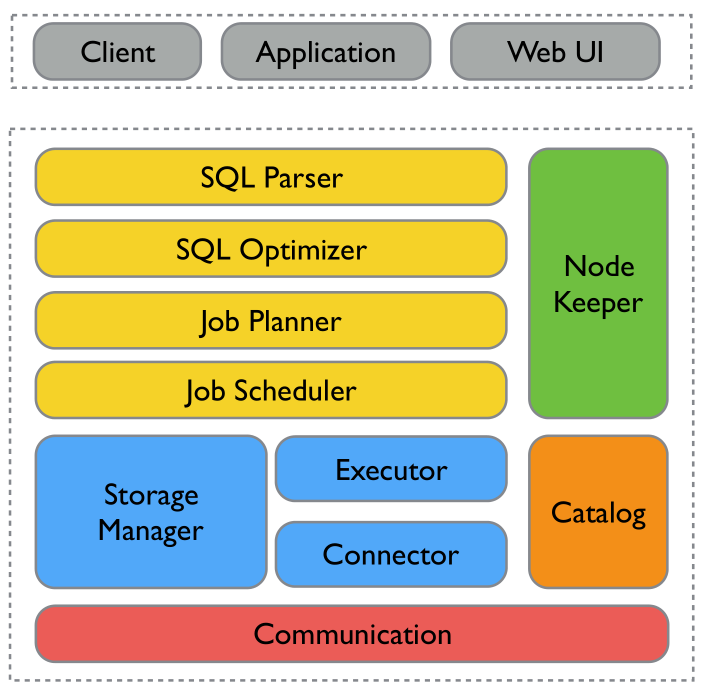
\includegraphics[width=0.7\linewidth]{figure/pard-node-in.png}
	\caption{Pard单个节点的架构}
	\label{fig:node1}
\end{figure}

\subsection{PardServer启动/关闭流程}
Pard Server的启动流程:
\begin{enumerate}
\item 初始化配置。读取配置文件,并且检查配置项。
\item 加载connector。加载配置的connector,包括初始化数据库JDBC连接的连接池。
\item 加载Catalog。初始化Catalog与etcd的连接,并启动etcd的watch线程。
\item 加载本地执行器(Executor)。初始化本地执行器。
\item 加载NodeKeeper。初始化本地的NodeKeeper模块。
\item 启动数据传输的ExchangeServer。以线程方式初始化和启动Netty。不阻塞主进程。
\item 启动文件传输的FileExchangeServer。以线程方式初始化和启动Netty。不阻塞主进程。
\item 启动RPCServer。以线程方式初始化和启动RPC服务。不阻塞主进程。
\item 加载JobScheduler。初始化JobScheduler,并创建单例。
\item 加载TaskScheduler。初始化TaskScheduler,并创建单例。
\item Pard Server注册。向NodeKeeper注册一个Pard Server,包括名称、IP地址、RPC端口、数据传输端口、文件传输端口等。该信息会在etcd中进行同步,方便其他节点查询。
\item 启动Pard Web Server。以线程方式启动内嵌的Jetty作为web server,目前用于展示查询计划。
\item 启动socket监听。服务器和客户端之间采用socket进行通信,启动服务器端的socket监听线程。
\item 注册shutdownHook。注册JVM进程停止的shutdownHook,该hook中添加的方法将会按照顺序在JVM停止之前执行,进行清理和资源释放。
\end{enumerate}

Pard Server的停止流程:
\begin{enumerate}
\item 停止web server。
\item 停止socket连接和监听。
\item 通知NodeKeeper更改Pard Server的状态为下线(或从NodeKeeper中删除该节点)。
\item 停止Catalog。中止etcd的watch线程,并释放与etcd的连接。
\item 停止本地执行器(Executor)。停止正在执行的task。
\item 停止数据传输的ExchangeServer。关闭Netty线程。
\item 停止文件传输的FileExchangeServer。关闭Netty线程。
\item 停止RPCServer。关闭RPC线程。
\item 关闭Connector。关闭与数据库的连接池。
\end{enumerate}

\subsection{时间安排}
如图\ref{fig:tl}。

\begin{figure}[htbp]
	\centering
	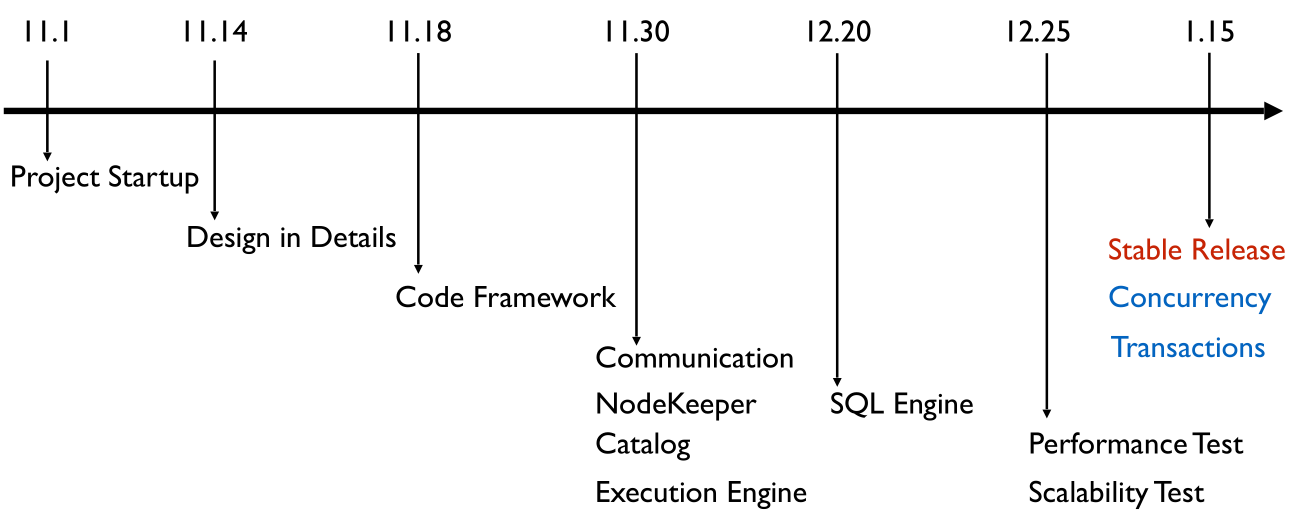
\includegraphics[width=\linewidth]{figure/timeline.png}
	\caption{时间安排timeline}
	\label{fig:tl}
\end{figure}

\section{各模块详细设计}
\subsection{执行流程}
package cn.edu.ruc.iir.pard.scheduler;

job 

ABORTED(0), BEGIN(1), PARSING(2), PLANNING(3), SCHEDULING(4), EXECUTING(5), DONE(6), FAILED(-1);


getNext() 状态转换



记录各个状态的job供用户查看。
private final List<Job> doneJobs;
private final List<Job> abortedJobs;
private final List<Job> failedJobs;


错误
cn.edu.ruc.iir.pard.planner.ErrorMessage



=============== 
package cn.edu.ruc.iir.pard.planner.ddl;
dml  优化具体 韩涵

\subsubsection{Insert/Delete 流程}
RPC

\subsubsection{Load 流程}
返回值比较少,返回状态

\subsubsection{Select 流程}


\subsubsection{Join 流程}



\subsection{节点通信}
通讯任务依据数据传输量的大小,和任务本身性质,可以自然的分为两类:


pipeline  Netty inbound outbound



\subsection{元数据}
元数据模型  etcd   


watch机制



\subsection{SQL解析}
语义语法解析
Antlrv4


\begin{lstlisting}
statement
: query                                                            #statementDefault
| USE schema=identifier                                            #use
| CREATE SCHEMA (IF NOT EXISTS)? qualifiedName                     #createSchema
| DROP SCHEMA (IF EXISTS)? qualifiedName (CASCADE | RESTRICT)?     #dropSchema
| ALTER SCHEMA qualifiedName RENAME TO identifier                  #renameSchema
| CREATE TABLE (IF NOT EXISTS)? qualifiedName
tableElementPart
(',' tableElementPart)*
partitionOps?                                                  #createTable
| CREATE INDEX indexName=identifier ON
indexTbl=qualifiedName '(' identifier (',' identifier)*')'     #createIndex
| DROP INDEX indexName=identifier                                  #dropIndex
| DROP TABLE (IF EXISTS)? qualifiedName                            #dropTable
| INSERT INTO qualifiedName columnAliases? query                   #insertInto
| DELETE FROM qualifiedName (WHERE booleanExpression)?             #delete
| ALTER TABLE from=qualifiedName RENAME TO to=qualifiedName        #renameTable
| ALTER TABLE tableName=qualifiedName
RENAME COLUMN from=identifier TO to=identifier                 #renameColumn
| ALTER TABLE tableName=qualifiedName
DROP COLUMN column=qualifiedName                               #dropColumn
| ALTER TABLE tableName=qualifiedName
ADD COLUMN column=columnDefinition                             #addColumn
| GRANT
(privilege (',' privilege)* | ALL PRIVILEGES)
ON TABLE? qualifiedName TO grantee=identifier
(WITH GRANT OPTION)?                                           #grant
| REVOKE
(GRANT OPTION FOR)?
(privilege (',' privilege)* | ALL PRIVILEGES)
ON TABLE? qualifiedName FROM grantee=identifier                #revoke
| SHOW GRANTS
(ON TABLE? qualifiedName)?                                     #showGrants
| EXPLAIN ANALYZE? VERBOSE?
('(' explainOption (',' explainOption)* ')')? statement        #explain
| SHOW STATS (FOR | ON) qualifiedName                              #showStats
| SHOW STATS FOR '(' querySpecification ')'                        #showStatsForQuery
| DESCRIBE qualifiedName                                           #showColumns
| DESC qualifiedName                                               #showColumns
| START TRANSACTION (transactionMode (',' transactionMode)*)?      #startTransaction
| COMMIT WORK?                                                     #commit
| ROLLBACK WORK?                                                   #rollback
| SHOW PARTITIONS (FROM | IN) qualifiedName                        #showPartitions
| SHOW SCHEMAS                                                     #showSchemas
| SHOW TABLES (FROM schemaName=identifier)?                        #showTables
| LOAD path=identifier INTO table=qualifiedName                    #load
;
\end{lstlisting}

支持基本的Select语句,如

select * from ASG where eno<’E1020’ and eno>=’E0990’


expression  and or not





\subsection{SQL优化}
% PLAN树结构
% PROJECT/FILTER下推
% 表达式计算
% INSERT/DELETE/SELECT剪枝
% JOIN优化

\section{任务分工及小结}

\subsection{金国栋的小结}

\subsection{韩涵的小结}

\subsection{黄文韬的小结}

\subsection{陈成的小结}





 
\end{document}